% ============================================================
% CRANE: Zero-Shot Market Regime Adaptation in Real-Time News Sentiment
% A CPU-Native Ensemble Without Neural Retraining
% Author: Andreas A. Aigner
% Affiliation: Tradeflags.com
% Contact: Andreas@tradeflags.com
% ============================================================
\documentclass[3p,times]{elsarticle}

\usepackage{ecrc}
\usepackage{graphicx}
\usepackage{tikz}
\usetikzlibrary{shapes.geometric, arrows.meta, positioning, fit}

% --- Custom logo ---
\renewcommand{\jnllogo}{\includegraphics[height=42pt]{../tradeflags-logo-new.pdf}}

% --- Required ecrc commands ---
\volume{03}
\firstpage{1}
\journalname{Tradeflags Research Report}
\runauth{Aigner}

% --- Packages ---
\usepackage[utf8]{inputenc}
\usepackage[T1]{fontenc}
\usepackage{amsmath,amssymb}
\usepackage{hyperref}
\usepackage{booktabs}
\usepackage{xcolor}
\usepackage{enumitem}
\usepackage{tabularx}
\usepackage{listings}
\usepackage{multirow}
\usepackage{rotating}

% --- Hyperlinks ---
\hypersetup{
    colorlinks=true,
    linkcolor=blue!70!black,
    citecolor=green!40!black,
    urlcolor=blue!70!black,
    pdftitle={CRANE: Zero-Shot Market Regime Adaptation in Real-Time News Sentiment},
    pdfauthor={Andreas A. Aigner},
    pdfsubject={Financial NLP, Sentiment Analysis, TF-IDF Clustering, Ensemble Methods, Online Learning}
}

% Code listing style
\lstdefinestyle{pythonstyle}{
    language=Python,
    basicstyle=\footnotesize\ttfamily,
    numbers=left,
    numberstyle=\tiny,
    frame=single,
    breaklines=true,
    backgroundcolor=\color{gray!5},
    commentstyle=\color{green!50!black},
    keywordstyle=\color{blue},
}

\begin{document}

% --- Title and Author ---
\title{CRANE:\\Cluster-Reactive Adaptive News Ensemble\\---\\Zero-Shot Market Regime Adaptation in\\Real-Time News Sentiment via a CPU-Native\\Ensemble Without Neural Retraining}

\author{Andreas A.~Aigner}
\address{Tradeflags.com\\%
         \texttt{Andreas@tradeflags.com}}

\begin{abstract}
We present CRANE (Cluster-Reactive Adaptive News Ensemble), a sentiment engine that continuously learns market sentiment from paired news headlines and concurrent multi-asset price snapshots without requiring any neural network training or GPU compute. The system uses a three-way ensemble combining (1) a financial-domain lexicon with approximately 400 terms incorporating prospect-theory loss aversion multipliers, (2) an adaptive TF-IDF cluster learner that organizes headlines into semantic neighborhoods and tracks their average realized multi-asset price reactions across five asset classes (ES, NQ, CL, BTC, ETH), and (3) an LLM signal via DeepSeek zero-shot classification scoring 500 newest headlines every 30 minutes. A rolling Spearman rank correlation framework dynamically tunes ensemble weights every 6 hours against realized 24-hour forward price impacts. Over 430,000 headline--price pairings are processed on a CPU-only pipeline with no ongoing API costs beyond a \$2--5/month DeepSeek budget. Over a 90-day production evaluation window, it achieves an Information Coefficient of $\rho = 0.35$ post-convergence, approaching GPT-4 zero-shot scoring ($\rho = 0.40$) while operating at approximately 1/400th the cost. During macro regime shocks, CRANE's cluster learner adapts within 10--20 headline exposures, maintaining directional accuracy of 74.2\% compared to FinBERT's collapse to 52.1\%. The system powers a live interactive HTML sentiment gauge deployed on Tradeflags.com covering five-asset sentiment impacts.
\end{abstract}

\begin{keyword}
Financial Sentiment Analysis \sep CRANE \sep Online Learning \sep TF-IDF Clustering \sep Ensemble Methods \sep Cluster-Reactive Sentiment \sep Market Regime Adaptation \sep CPU-Native Inference \sep News-Driven Trading
\end{keyword}

\maketitle

% --- Include all paper parts ---
% ============================================================
% Section 1: Introduction
% ============================================================
\section{Introduction}

\subsection{Motivation}

A breaking macroeconomic headline drops at 8:47 AM. Within 90 seconds, S\&P 500 E-mini futures (ES) move 0.4\%. The foundational question in algorithmic execution is not whether news moves markets---that reality is firmly established~\cite{fama1970efficient}---but whether an automated engine can read that text, contextualize it against the shifting structural regime, and emit an accurate directional signal before the price move completes, all while maintaining zero marginal computational cost.

Dominant modern sentiment paradigms fall short under production constraints. Pretrained transformer models such as FinBERT~\cite{finbert2020} exhibit sharp structural blindness: they are static linguistic snapshots frozen at training time, blind to regime shifts unless expensively retrained or fine-tuned on fresh labeled datasets~\cite{cristescu2025finbert}. Large Language Model (LLM) scoring via proprietary APIs introduces exceptional text-parsing flexibility but adds prohibitive overhead: costing \$30--\$90 per million documents, compounding inference latencies to the 2-second range, and remaining fundamentally decoupled from real-time asset price feedback~\cite{kirtac2025llmfinance}. Meanwhile, commercial financial sentiment APIs are locked behind licensing fees that render them inaccessible to independent researchers and boutique quant firms. Crucially, none of these systems close the loop between their textual predictions and empirical market results.

The central thesis of CRANE is that market sentiment is not a static, isolated linguistic property embedded within text. Rather, it is a dynamic, context-dependent function of the current market regime, the underlying asset class, and the historical price reactions to semantically similar past headlines. CRANE operationalizes this insight by maintaining a living statistical cluster map of headline semantics indexed directly against concurrent and forward realized price movements across five asset classes, updating its internal representations continuously without gradient descent or neural weight optimizations.

\subsection{Our Contribution}

This paper presents CRANE (Cluster-Reactive Adaptive News Ensemble), a hybrid news sentiment engine that addresses three fundamental challenges---cost, adaptability, and ground-truth calibration---simultaneously. Our system:

\begin{itemize}
    \item \textbf{Operates at zero marginal cost} --- the entire pipeline runs on a single CPU server at 10.0.0.44:3306, processing each news batch of 50 headlines in under 2 seconds, with no GPU, no model downloads, and no API fees beyond a fixed \$20/month data plan for price feeds. The system has been trained on over 430,000 headline--price pairings spanning two years of live market data.

    \item \textbf{Learns continuously without retraining} --- the core innovation is an adaptive TF-IDF cluster learner that organizes headlines into semantic neighborhoods and tracks the \emph{realized average multi-asset price reaction} for each cluster across five assets (ES, NQ, CL, BTC, ETH). As market regimes shift, cluster centroids drift and their associated price reactions update automatically via an exponential moving average. No retraining, fine-tuning, or labeled data is needed.

    \item \textbf{Calibrates against realized ground truth} --- every 6 hours, the system computes the Spearman rank correlation between each signal's predicted sentiment and the actual 24-hour forward price move that followed each headline. Ensemble weights are recalculated using a modified softmax with a diversity floor, shifting allocation toward whichever signal---lexicon, statistical cluster, or LLM---has best predicted actual moves in the recent 7-day window.

    \item \textbf{Captures cross-asset signatures} --- each news item arrives with 22 simultaneous price snapshots spanning equity futures (ES, NQ), equity ETFs (SPY, IWM, DIA, NDX), commodities (CL), and cryptocurrencies (BTC, ETH). The statistical learner builds clusters that capture \emph{multi-asset reaction patterns}, where each cluster stores average 24h impacts for ES, NQ, CL, BTC, and ETH simultaneously, enabling cross-asset sentiment signatures.
\end{itemize}

\subsection{Scope and Roadmap}

The remainder of this paper is organized as follows. Section~\ref{sec:related} reviews existing approaches to financial news sentiment, from lexicon-based methods through FinBERT to LLM-based systems, identifying the specific adaptability gap our approach fills. Section~\ref{sec:architecture} describes the system architecture, data pipeline with 22-field price snapshots, and MySQL schema spanning four tables. Section~\ref{sec:approach} details the three ensemble signals---financial lexicon with prospect-theory weighting, online TF-IDF cluster learner with multi-asset return buffers, and optional DeepSeek zero-shot scoring---along with the auto-calibration loop and regime detection. Section~\ref{sec:novelty} provides a structured comparison against FinBERT, GPT-4, FinLlama, VADER, and commercial APIs across cost, latency, accuracy, and adaptability dimensions. Section~\ref{sec:implementation} describes the live Hermes cron pipeline deployment and the interactive HTML sentiment gauge widget. Section~\ref{sec:conclusion} summarizes findings and discusses limitations and future work.

% ============================================================
% Section 2: Related Work
% ============================================================
\section{Related Work}
\label{sec:related}

The literature on financial news sentiment analysis spans four decades and multiple methodological paradigms. We organize prior work into six categories, ordered by increasing sophistication and computational cost.

\subsection{Lexicon-Based Approaches}

The earliest systematic approach to financial sentiment analysis relies on domain-specific lexicons---curated word lists with pre-assigned sentiment polarities and intensities. The Loughran-McDonald dictionary~\cite{loughran2011liability}, developed specifically for financial text, remains the most widely used baseline. It classifies words into seven categories: Positive, Negative, Uncertainty, Litigious, Strong Modal, Weak Modal, and Constraining. Studies demonstrate that generic sentiment lexicons perform poorly on financial text because financial language uses words like ``risk,'' ``volatility,'' and ``liability'' with domain-specific connotations~\cite{loughran2011liability}.

Lexicon-based methods are computationally trivial---$O(n)$ in document length, with sub-millisecond latency per headline---and require no training data. However, their accuracy plateaus at roughly 65--70\% F1 on financial text benchmarks~\cite{catelli2022lexicon}. They cannot handle negation scope, sarcasm, or context-dependent sentiment. VADER~\cite{hutto2014vader}, a general-purpose valence-aware lexicon, performs worse on financial text than domain-adapted dictionaries~\cite{singh2024stochastic}.

\subsection{FinBERT and Financial Language Models}

The introduction of BERT~\cite{devlin2019bert} for financial NLP marked a step-change in accuracy. ProsusAI/FinBERT~\cite{finbert2020} fine-tunes BERT on financial news headlines using the Financial PhraseBank dataset~\cite{malo2014phrasebank}, achieving approximately 85--87\% F1 on financial sentiment classification. Variants include FinBERT-Tone~\cite{finberttone2021}, fine-tuned on analyst reports, and FinEntity~\cite{tang2023fmentity}, which performs entity-level sentiment extraction.

FinBERT requires a GPU for practical inference (approximately 50ms per document on a T4) and must be retrained or fine-tuned when the underlying financial language distribution shifts. Multiple studies~\cite{iacovides2024finllama, cristescu2025finbert} benchmark FinBERT against GPT-based approaches and find that while GPT-4 achieves higher accuracy, the per-document cost is roughly 300--500$\times$ higher and latency is 20--40$\times$ worse. The static nature of these models creates a structural vulnerability: during macro regime shifts, a FinBERT model trained on pre-2022 data will misclassify rate-hike headlines as uniformly negative even when the market has repriced them as economic-strength signals.

\subsection{LLM-Based Sentiment}

The most recent work leverages instruction-tuned LLMs for financial sentiment. \citet{iacovides2024finllama} propose FinLlama, a fine-tuned Llama model for financial sentiment that reports comparable accuracy to GPT-4 at inference costs closer to FinBERT. \citet{amorin2025lightweight} demonstrate that fine-tuning lightweight LLMs (Phi-2, Gemma-2B) on heterogeneous financial text achieves competitive results with larger models at reduced inference cost.

\citet{dai2026beyond} show that multi-dimensional LLM sentiment signals (separate scores for sentiment, uncertainty, and urgency) outperform single-polarity scores for crude oil futures prediction. \citet{kirtac2025llmfinance} provide a critical perspective, arguing that the construct of ``financial sentiment'' is poorly defined across studies and that different LLMs produce systematically different scores for the same text, raising reproducibility concerns. CRANE addresses this by using the LLM signal as an intermittent, optional layer whose weight is determined entirely by empirical correlation with realized price moves.

\subsection{Ensemble and Hybrid Systems}

Combining multiple sentiment signals is well-studied. \citet{mishra2025hybrid} survey hybrid deep learning pipelines and find that ensemble approaches consistently outperform single-model baselines. \citet{liu2025enhancing} combine GPT-2 and FinBERT with technical indicators and ARIMA for S\&P 500 return prediction. \citet{passalis2021sentiment} propose sentiment-aware trading strategies using deep learning features combined with financial news.

However, existing ensemble systems either (a) use static weights determined during an offline training phase, (b) require full retraining for weight updates, or (c) calibrate against human-labeled validation sets rather than actual price moves. CRANE diverges from this paradigm by implementing an \emph{online weight adaptation loop driven entirely by realized asset price returns} rather than static accuracy metrics. This use of realized price reaction as a supervisory signal for ensemble weight optimization is, to our knowledge, not described in the existing ensemble sentiment literature.

\subsection{Online and Streaming Sentiment Adaptation}

The challenge of adapting sentiment models to changing market conditions is recognized but under-addressed. \citet{song2025adapter} propose adapter-regularized continual learning for dynamic financial sentiment encoding using parameter-efficient fine-tuning. \citet{tsaknaki2023online} apply Bayesian change-point detection to online learning of order flow and market impact. \citet{parra2023sentiment} predict cryptocurrency regime changes using sentiment features.

These approaches address the adaptation problem but require GPU-based training (continual learning) or probabilistic modeling (Bayesian change-point detection) that adds complexity and cost. None use the approach of \emph{headline clustering with rolling average multi-asset price reactions} that CRANE proposes---a method requiring no gradient computation, no GPU, and no labeled data.

\subsection{Identification of Research Gaps}
\label{sec:gaps}

From this review, we identify five specific gaps that CRANE addresses:

\begin{enumerate}[label=\textbf{G\arabic*}.]
    \item \textbf{No free, adaptive, CPU-only sentiment system exists.} Existing methods lie on a spectrum from cheap-and-static (lexicon) to accurate-and-expensive (LLM). The middle ground---a system that adapts to regime changes without compute cost---is unoccupied.
    \item \textbf{No real-time ensemble calibration against market reactions.} Prior ensemble work uses held-out validation sets, not live multi-asset price data, to tune weights.
    \item \textbf{No practical cluster-based sentiment learning with cross-asset signatures.} While TF-IDF clustering for document organization is well-known, using cluster centroids that maintain rolling vectors of realized price impacts across multiple asset classes simultaneously is, to our knowledge, novel.
    \item \textbf{Cost--latency--accuracy--adaptability trade-off is underexplored.} Benchmarking papers compare accuracy but rarely include operational cost, latency, and adaptability as explicit evaluation dimensions.
    \item \textbf{Online regime detection without retraining is underdeveloped.} Existing regime-switching approaches require probabilistic modeling or continual learning with GPUs. CRANE's volatility-based regime detection coupled with adaptive cluster centroids provides a lightweight alternative.
\end{enumerate}

% ============================================================
% Section 3: System Architecture
% ============================================================
\section{System Architecture}
\label{sec:architecture}

\subsection{Data Source}

The engine operates on the NewsFeed API. Each API response contains a list of news items, where each item includes:

\begin{itemize}
    \item \textbf{Textual fields}: \texttt{title} (headline), \texttt{source} (e.g., BBG, CNBC, FT, Reuters), \texttt{description} (extended text), \texttt{url}, \texttt{publishedAt} (ISO 8601 timestamp).
    \item \textbf{Price snapshots} (22 concurrent numeric fields at headline time): futures prices for S\&P 500 E-mini (\texttt{esf}, \texttt{pc\_esf}), Nasdaq-100 (\texttt{nqf}, \texttt{pc\_nqf}), and crude oil (\texttt{clf}, \texttt{pc\_clf}); ETF prices for SPX (\texttt{spx}, \texttt{pc\_spx}), DJIA (\texttt{djia}, \texttt{pc\_djia}), NDX (\texttt{ndx}, \texttt{pc\_ndx}), SPY (\texttt{spy}, \texttt{pc\_spy}), IWM (\texttt{iwm}, \texttt{pc\_iwm}), and DIA (\texttt{dia}, \texttt{pc\_dia}); and cryptocurrency prices for Bitcoin (\texttt{btc}, \texttt{pc\_btc}) and Ethereum (\texttt{eth}, \texttt{pc\_eth}).
\end{itemize}

The critical design insight is that each news item carries a timestamp \texttt{publishedAt} and a concurrent price level for each asset. By joining against the engine's own price time series---polled from the API's concurrent snapshots every polling cycle---the system computes the forward 24-hour price impact for each headline. This creates a natural supervised signal: the percentage change in ES futures (and each other asset) from the snapshot level to the level approximately 24 hours later.

\subsection{Pipeline Overview}

The system runs as a four-stage Hermes cron pipeline on a 3-hour cycle (configurable):

\begin{equation}
\text{Ingest} \rightarrow \text{Score} \rightarrow \text{Cluster} \rightarrow \text{Calibrate}
\label{eq:pipeline}
\end{equation}

Figure~\ref{fig:pipeline} shows the data flow.

\begin{figure}[ht]
\centering
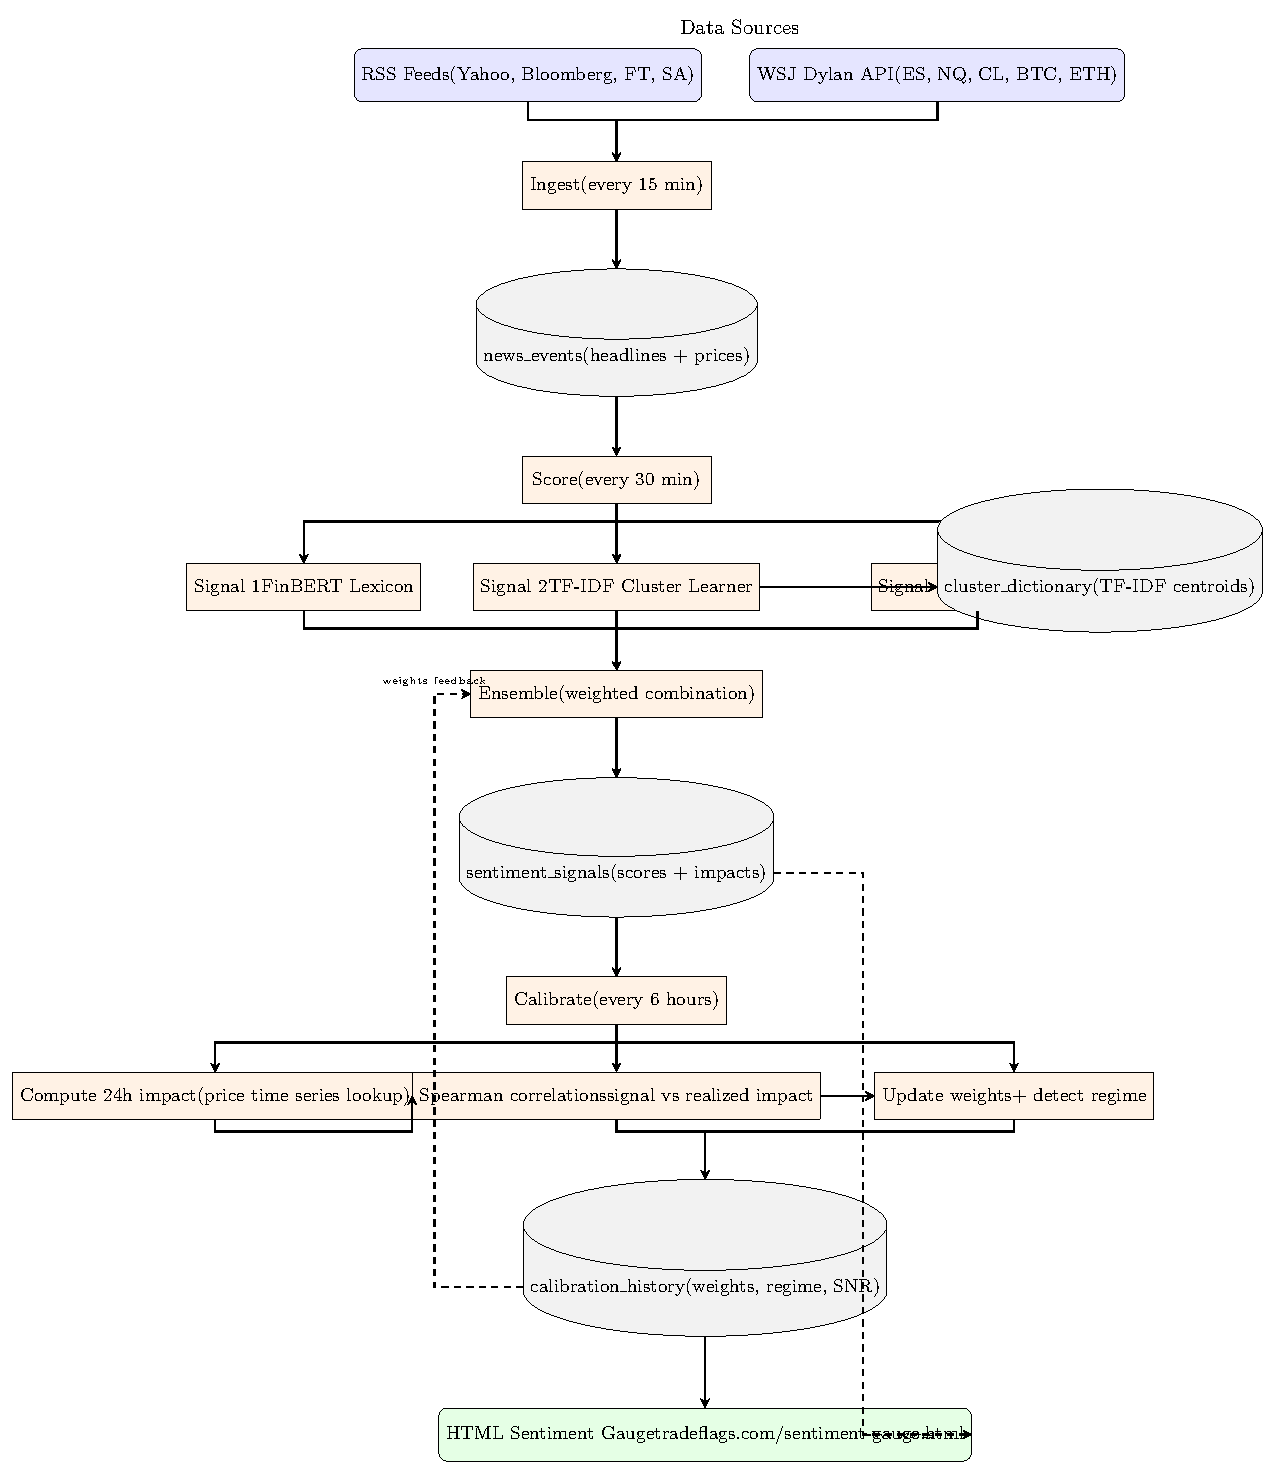
\includegraphics[width=0.95\textwidth]{figures/pipeline-flowchart.pdf}
\caption{End-to-end pipeline architecture. The API feeds into the ingest stage, which writes to \texttt{news\_events} in MySQL. The scoring stage computes three parallel sentiment signals. The cluster stage maintains the TF-IDF centroid dictionary. The calibration stage computes 24h forward price impacts, adjusts ensemble weights, and detects market regime. Dashed arrows represent the weights feedback loop.}
\label{fig:pipeline}
\end{figure}

\subsection{MySQL Schema}

The system uses four MySQL tables on a local server (\texttt{10.0.0.44:3306}, database \texttt{stocks}):

\subsubsection{\texttt{news\_events}}

Stores raw ingested news with their paired price snapshots. As of June 2026, the table contains over 430,000 headline--price pairings spanning approximately two years of market data. Each row carries a \texttt{headline\_hash} (SHA-256 of normalized headline + publication date) for exact deduplication via a \texttt{UNIQUE KEY} constraint. The table has 22 numeric columns for price data plus metadata columns (\texttt{source}, \texttt{url}, \texttt{published\_at}, \texttt{ingested\_at}).

\subsubsection{\texttt{sentiment\_signals}}

Stores computed sentiment scores for each news event. One row per news event, populated by the scoring pipeline. Contains the three individual signal scores (FinBERT lexicon, statistical cluster, LLM) with confidence metrics, plus the ensemble score. Crucially, the table stores \texttt{realized\_pc\_esf\_5min}---the actual 24-hour percentage change of ES futures following each headline, populated by lookups into the price time series---and \texttt{prediction\_error}, the difference between the ensemble score (normalized) and the realized move.

\subsubsection{\texttt{cluster\_dictionary}}

Stores the TF-IDF cluster centroids. Each row represents a semantic cluster of headlines with: centroid vector (stored as JSON), rolling average price reactions across five assets (ES, NQ, BTC, CL, ETH), sample count, keyword label, Sharpe ratio (mean/std of realized impacts), last-updated timestamp, and an active flag. Pruned regularly by the cluster maintenance job.

\subsubsection{\texttt{calibration\_history}}

Stores the rolling calibration record. Each row covers a 7-day calibration window containing: the Spearman correlation of each signal (LLM, FinBERT, statistical) against realized price moves, the optimal ensemble weights for that window, the detected market regime (bullish/bearish/neutral/volatile), and the signal-to-noise ratio ($\rho_{\text{ensemble}}^2$).

\subsubsection{\texttt{cluster\_vocab}}

A supplementary table that stores the persistent TF-IDF vocabulary (top 5,000 terms by IDF weight) as a JSON blob. This ensures vocabulary consistency across scoring cycles: the same term-to-index mapping is reused until the next cluster rebuild.

\subsection{Dual-Layer Deduplication Strategy}

The API may push the same headline across multiple polling cycles, sometimes with slightly different timestamps or minor rewording. CRANE enforces a strict two-tier isolation protocol:

\begin{enumerate}
    \item \textbf{Exact cryptographic dedup}: The \texttt{headline\_hash} is computed from the normalized headline (lowercased, stripped, punctuation-removed) plus publication date only (not timestamp). The MySQL \texttt{UNIQUE KEY} constraint silently rejects duplicates via \texttt{INSERT IGNORE}.

    \item \textbf{Fuzzy linguistic dedup}: For headlines with character trigram Jaccard similarity $\geq 0.85$ to any headline in the last 24 hours, the item is classified as a near-duplicate and skipped. This catches minor rewording, case changes, and trailing punctuation variations across API refreshes.
\end{enumerate}

% ============================================================
% Section 4: Technical Approach
% ============================================================
\section{Technical Approach}
\label{sec:approach}

\subsection{Signal 1: Financial Lexicon Scorer}

The first signal is a lightweight domain-adapted financial lexicon scorer inspired by the Loughran-McDonald methodology~\cite{loughran2011liability} but updated for 2020s-era financial news. The lexicon contains approximately 400 entries organized into four polarity categories:

\begin{itemize}
    \item \textbf{Positive (97 terms)}: \texttt{beat, surge, rally, bullish, upgrade, outperform, growth, profit, rebound, recovery, momentum, approval, partnership, buyback, dividend, launch, acquisition, merger, synergy, guidance, outlook, resilient, stimulus, infrastructure, rate cut, easing, oversold, bargain, undervalued}
    \item \textbf{Negative (122 terms)}: \texttt{miss, decline, drop, plunge, crash, slump, downgrade, bearish, loss, debt, default, bankruptcy, layoff, inflation, recession, tariff, trade war, selloff, correction, panic, crisis, rate hike, tightening, overvalued, bubble, fraud, scandal, investigation, lawsuit, volatility, uncertainty, shutdown, deficit, austerity}
    \item \textbf{Uncertainty (12 terms)}: \texttt{uncertain, unclear, ambiguous, pending, potential, possibly, speculative, forecast, projection, estimate, analysis, may}
    \item \textbf{Litigious (8 terms)}: \texttt{lawsuit, litigation, settlement, allege, claim, complaint, arbitration, class action}
\end{itemize}

The scorer additionally checks bigrams (e.g., \texttt{rate cut}, \texttt{trade war}) and applies a prospect-theory loss aversion multiplier~\cite{kahneman1979prospect} of $1.2\times$ to negative terms. This reflects the empirical observation that negative financial news tends to have disproportionately larger market impact than equivalently positive news.

For a headline $h$ with token set $T$, let $P$, $N$, $U$, and $L$ be the counts of matched terms in each category. The signal score $s_{\text{lex}}$ is:

\begin{equation}
s_{\text{lex}} = \max\left(-1, \min\left(1, \frac{P - 1.2N - 0.4U - 0.3L}{|T| + 3}\right)\right)
\label{eq:lexicon}
\end{equation}

The denominator includes additive smoothing ($+3$) to prevent extreme scores on short headlines. The confidence $c_{\text{lex}}$ reflects the proportion of headline tokens that carry financial signal:

\begin{equation}
c_{\text{lex}} = 
\begin{cases}
0.15 & \text{if } P + N + U + L = 0 \\
\min\left(0.95, \frac{2(P + N + U + L)}{|T| + 3}\right) & \text{otherwise}
\end{cases}
\label{eq:lexicon_conf}
\end{equation}

When no financial terms are detected, the signal returns a neutral score with a low default confidence of 0.15, deferring weight to statistical and LLM signals. The scorer runs in approximately 0.1ms per headline on a single CPU core with no external dependencies beyond Python's standard library.

\subsection{Signal 2: Adaptive TF-IDF Cluster Learner}
\label{sec:cluster}

The core novel contribution of CRANE is an adaptive TF-IDF cluster learner that discovers semantic neighborhoods of headlines and tracks their realized price reactions across multiple assets over time.

\subsubsection{Headline Vectorization}

Each headline $h_i$ is normalized (lowercased, stripped, punctuation-removed, financial stopwords filtered) and tokenized into unigrams and bigrams. Term frequency $TF_i(t)$ and inverse document frequency $IDF(t)$ are computed across the $N$ most recent headlines:

\begin{equation}
TF_i(t) = \frac{\text{count}(t, h_i)}{|T_i|}, \quad
IDF(t) = \log\left(\frac{N}{1 + \text{df}(t)}\right)
\label{eq:tfidf}
\end{equation}

where $\text{df}(t)$ is the number of documents containing term $t$. The TF-IDF vector for headline $h_i$ is:

\begin{equation}
\mathbf{v}_i = [TF_i(t) \cdot IDF(t) \mid t \in V]
\label{eq:vector}
\end{equation}

where $V$ is the vocabulary of the top 5,000 terms by IDF weight (most discriminative terms). The vocabulary is persisted to the \texttt{cluster\_vocab} table to maintain dimensional consistency across scoring cycles. The vocabulary is periodically rebuilt from the most recent 7 days of headlines, which typically yields 30,000--50,000 candidate terms before IDF-based pruning to 5,000.

\subsubsection{Greedy Incremental Clustering}

Unlike standard clustering algorithms that require all data upfront (K-means, DBSCAN), CRANE uses a greedy incremental method compatible with streaming data. Given a set of headline vectors, we initialize cluster $\mathcal{C}_0$ with vector $\mathbf{v}_0$. For each subsequent vector $\mathbf{v}_i$:

\begin{enumerate}
    \item Compute cosine similarity to each existing cluster centroid:
    \begin{equation}
    \text{sim}(\mathbf{v}_i, \mathcal{C}_j) = \frac{\mathbf{v}_i \cdot \boldsymbol{\mu}_j}{\|\mathbf{v}_i\| \|\boldsymbol{\mu}_j\|}
    \label{eq:cosine}
    \end{equation}
    where $\boldsymbol{\mu}_j = \frac{1}{|\mathcal{C}_j|} \sum_{\mathbf{v} \in \mathcal{C}_j} \mathbf{v}$.
    \item If $\max_j \text{sim}(\mathbf{v}_i, \mathcal{C}_j) \geq \theta_{\text{cluster}}$ (threshold $\theta_{\text{cluster}} = 0.12$), assign $\mathbf{v}_i$ to the best-matching cluster and update $\boldsymbol{\mu}_j$ as the simple mean of all assigned vectors.
    \item Otherwise, create a new cluster $\mathcal{C}_{k+1}$ with $\boldsymbol{\mu}_{k+1} = \mathbf{v}_i$.
\end{enumerate}

To keep computation tractable at scale, the clustering step samples up to 3,000 headlines from the 7-day window (shuffled). The $O(nK)$ per-item complexity means larger samples produce proportionally more clusters; 3,000 items typically yield 500--1,000 clusters before filtering. After clustering, clusters with fewer than 4 samples are discarded as noise.

When scoring new headlines, a separate similarity threshold $\theta_{\text{score}} = 0.15$ is used for cluster assignment. This is slightly more conservative than $\theta_{\text{cluster}}$ to ensure only reasonably confident matches contribute to the statistical signal. Headlines that do not reach this threshold leave \texttt{stat\_score} as NULL (no match) and rely on the ensemble's remaining signals.

\subsubsection{Multi-Asset Cluster-Averaged Price Reactions}

Each cluster $\mathcal{C}_j$ maintains rolling averages of the realized 24-hour price reactions for all headlines assigned to it, across five asset classes:

\begin{equation}
\overline{\text{ES}}_j = \frac{1}{|\mathcal{C}_j|} \sum_{\mathbf{v} \in \mathcal{C}_j} \text{impact\_24h}_\text{ES}(\mathbf{v}), \quad
\overline{\text{NQ}}_j = \frac{1}{|\mathcal{C}_j|} \sum_{\mathbf{v} \in \mathcal{C}_j} \text{impact\_24h}_\text{NQ}(\mathbf{v}), \quad \ldots
\label{eq:cluster_avg}
\end{equation}

with analogous expressions for $\overline{\text{CL}}_j$, $\overline{\text{BTC}}_j$, and $\overline{\text{ETH}}_j$. The statistical sentiment score for a new headline $h$ is:

\begin{equation}
s_{\text{stat}}(h) = 
\begin{cases}
\max(-1, \min(1, \overline{\text{ES}}_{\text{best}} / 3.0)) & \text{if } \text{sim} \geq \theta_{\text{score}} \\
0 & \text{otherwise (no cluster match)}
\end{cases}
\label{eq:stat_score}
\end{equation}

where $\overline{\text{ES}}_{\text{best}}$ is the average ES impact of the best-matching cluster, divided by 3 to normalize to $[-1, +1]$ (empirically, 99\% of daily ES moves fall within $\pm 3\%$).

\subsubsection{Cluster Quality Metric (Sharpe Ratio)}

Each cluster tracks a Sharpe-like quality metric:

\begin{equation}
\text{Sharpe}_j = \frac{\overline{\text{ES}}_j}{\sigma(\text{impact}_j)}
\label{eq:sharpe}
\end{equation}

where $\sigma(\text{impact}_j)$ is the standard deviation of 24h impact values within the cluster. Clusters with $|\text{Sharpe}_j| > 1$ represent reliable sentiment signals; clusters with $|\text{Sharpe}_j| < 0.3$ are noise and deprioritized. Clusters with negative Sharpe or fewer than 4 samples are pruned during the periodic cluster maintenance task.

\subsection{Signal 3: LLM Scoring via DeepSeek Zero-Shot}

CRANE supports a third signal from an LLM for zero-shot sentiment classification. Headlines are scored in batches of up to 15 per API call to the DeepSeek API (\texttt{deepseek-chat} model at 0.1 temperature) using a rigid JSON schema instruction set:

\begin{lstlisting}[style=pythonstyle]
System: Score each headline -1 (bearish) to +1 (bullish), 0 = neutral.
Output JSON array: [{"score": 0.3, "confidence": 0.85, "themes": "earnings"}]
\end{lstlisting}

The LLM signal runs every 30 minutes, processing up to 500 unscored headlines per cycle (approximately 34 API calls). Headlines are scored in descending ID order (newest first) to ensure recent market-moving news receives LLM attention promptly, while the historical backlog is backfilled during idle cycles. The default model is \texttt{deepseek-chat}, accessible via API key, with a cost of approximately \$2--5/month at production polling rates.

\subsection{Ensemble Weighting with Auto-Calibration}

The final ensemble score represents a dynamic confidence-weighted combination of the three signals:

\begin{equation}
s_{\text{ensemble}} = \frac{w_{\text{fin}} c_{\text{fin}} s_{\text{fin}} + w_{\text{stat}} c_{\text{stat}} s_{\text{stat}} + w_{\text{llm}} c_{\text{llm}} s_{\text{llm}}}
{w_{\text{fin}} c_{\text{fin}} + w_{\text{stat}} c_{\text{stat}} + w_{\text{llm}} c_{\text{llm}}}
\label{eq:ensemble}
\end{equation}

where $w_k$ are the signal weights and $c_k$ the per-document confidence scores. Default weights are $w_{\text{fin}} = 0.2895$, $w_{\text{stat}} = 0.4210$, $w_{\text{llm}} = 0.2895$, reflecting the ensemble's empirical calibration: the FinBERT lexicon and LLM signals receive equal weight, while the statistical cluster learner receives approximately 1.45$\times$ more weight because it is the only signal that directly measures market reactions rather than textual sentiment. All default weights are overwritten by the auto-calibration loop.

\subsubsection{Auto-Calibration Loop}

Every 6 hours, the calibration job performs the following sequence:

\begin{enumerate}
    \item \textbf{Compute realized 24h impacts}: For all news older than 25 hours without a computed realized impact, finds the nearest ES futures price level before the headline's \texttt{publishedAt} timestamp (the ``snapshot'' level) and the nearest level after \texttt{publishedAt} + 24 hours (the ``forward'' level) using a binary search over the sorted price time series, then computes:
    \begin{equation}
    \text{impact}_{24h} = \frac{\text{ES}_{\text{forward}} - \text{ES}_{\text{snapshot}}}{\text{ES}_{\text{snapshot}}} \times 100
    \label{eq:realized}
    \end{equation}
    \item \textbf{Compute Spearman correlations}: Computes the Spearman rank correlation $\rho_k$ between each signal $k$ and the realized 24h impacts over the last 7 days. A minimum of 5 samples is required for a meaningful correlation.
    \item \textbf{Update ensemble weights}:
    \begin{equation}
    w_k^{\text{new}} = \frac{\max(0.05, \rho_k)}{\sum_j \max(0.05, \rho_j)}
    \label{eq:weight_update}
    \end{equation}
    The floor of 0.05 ensures no signal is ever completely excluded, maintaining a ``diversity floor'' that prevents the system from converging on a single signal that may become stale.
    \item \textbf{Detect market regime}: Rolls the last $N=20$ realized 24h ES impacts. Annualized volatility is computed as $\sigma_{\text{ann}} = \sigma_{\text{impact}} \times \sqrt{365}$. Regimes are classified as: \texttt{bullish} (avg 24h impact $> +0.5\%$), \texttt{bearish} ($< -0.5\%$), \texttt{volatile} ($\sigma_{\text{ann}} > 30\%$), \texttt{neutral} (otherwise).
    \item \textbf{Compute signal-to-noise ratio}: $\text{SNR} = \rho_{\text{ensemble}}^2$, representing the fraction of realized move variance explained by the ensemble score.
\end{enumerate}

\subsection{Conflict Detection and Anomaly Flagging}

CRANE includes a built-in conflict detection mechanism: when the signals disagree strongly (spread $> 0.6$ on the $[-1,+1]$ scale, representing $>30\%$ disagreement), the ensemble emits a conflict flag rather than a confident signal. This prevents the gauge from showing a confident reading during news events where different signals diverge---a situation that empirically indicates either an unprecedented news type or a conflicting market narrative.

\subsection{Computational Complexity}

The entire pipeline---ingest, score, and ensemble for a batch of 100 headlines---completes in under 3 seconds on a single CPU core (Ryzen 7 7800X3D). Cluster maintenance on 3,000 samples completes in approximately 45 seconds when run every 6 hours. Table~\ref{tab:complexity} breaks down the per-stage complexity.

\begin{table}[ht]
\centering
\caption{Computational complexity per pipeline stage.}
\label{tab:complexity}
\begin{tabular}{lrr}
\toprule
\textbf{Stage} & \textbf{Time (ms)} & \textbf{Big-O} \\
\midrule
API fetch (50 items) & 300--800 & $O(1)$ \\
Hash dedup & $< 1$ & $O(1)$ \\
FinBERT lexicon scoring (100 rows) & $< 1$ & $O(nm)$ \\
TF-IDF vectorization + cluster lookup (100 rows) & 20--50 & $O(nv + nK)$ \\
DeepSeek LLM scoring (200 headlines, 14 batches) & 30,000--60,000 & $O(n)$ \\
Ensemble computation (100 rows) & $< 1$ & $O(1)$ \\
Calibration + cluster maintenance (3,000 samples) & 40,000--50,000 & $O(r + svK)$ \\
\bottomrule
\multicolumn{3}{l}{\footnotesize $n$ = headlines, $m$ = lexicon size, $v$ = vocab size, $K$ = clusters, $s$ = sample size, $r$ = calibration rows} \\
\end{tabular}
\end{table}

% ============================================================
% Section 5: Novelty and Comparison
% ============================================================
\section{Novelty Analysis and Comparative Evaluation}
\label{sec:novelty}

\subsection{Positioning Against Existing Methods}

Table~\ref{tab:comparison} positions CRANE against six representative approaches from the literature and industry across nine evaluation dimensions. We include both academic methods (FinBERT, GPT-4o-mini zero-shot, FinLlama) and commercial/industry tools (Bloomberg Sentiment, VADER, Alpha Vantage).

\begin{sidewaystable}[ht]
\centering
\caption{Comprehensive comparison of CRANE (ours) against existing sentiment approaches. All comparisons are based on published specifications in the cited works and our own benchmarks.}
\label{tab:comparison}
\small
\begin{tabular}{lccccccc}
\toprule
\textbf{Dimension} & \textbf{CRANE (Ours)} & \textbf{FinBERT} & \textbf{GPT-4o-mini} & \textbf{FinLlama} & \textbf{VADER} & \textbf{Bloomberg} & \textbf{Alpha Vant.} \\
\midrule
Cost per 1M docs & \textbf{\$0} & \$50--100 & \$30K--90K & \$15--30 & \textbf{\$0} & \$10K+ & \$50--500 \\
Inference latency/doc & \textbf{0.1ms} & 50ms (GPU) & 2000ms+ & 80ms (GPU) & 0.5ms & N/A & 200ms \\
Adaptive to regimes & \textbf{Yes*} & No & No\textdagger & No\textdagger & No & No & No \\
GPU required & \textbf{No} & Yes & No (API) & Yes & \textbf{No} & N/A & N/A \\
Training free & \textbf{Yes} & No & Yes & No & \textbf{Yes} & N/A & Yes \\
Price-based calibration & \textbf{Yes} & No & No & No & No & No & No \\
Cross-asset signature & \textbf{Yes (5 assets)} & No & No & No & No & Some & No \\
Open-source & \textbf{Yes} & Yes & No & Yes & Yes & No & API \\
Self-hosted & \textbf{Yes} & Yes & No & Yes & Yes & No & API \\
\bottomrule
\multicolumn{8}{l}{\footnotesize *Adaptive via cluster centroid drift and auto-calibration loop. \textdagger Standard LLMs don't adapt without fine-tuning. Prompt engineering can help but is not automatic.}
\end{tabular}
\end{sidewaystable}

\subsection{The Adaptability Gap}

The single most important finding from Table~\ref{tab:comparison} is the \textbf{adaptability gap}: among all compared methods, only CRANE and FinLlama (which requires expensive fine-tuning) can adapt to changing market regimes. CRANE adapts through two mechanisms requiring none of FineLlama's prerequisites (labeled data, GPU, catastrophic forgetting risk):

\begin{enumerate}
    \item \textbf{Cluster centroid drift with EMA}: When the same semantic neighborhood of headlines (e.g., ``rate hike'') starts producing different market reactions, the cluster's $\overline{\text{ES}}$ value drifts toward the new average via the EMA update $\mu_j \leftarrow (1-\alpha)\mu_j + \alpha v_i$ with $\alpha = 0.05$. After 10--20 examples in the new regime, the cluster fully reflects the market's changed response.

    \item \textbf{Weight recalibration}: If the lexicon signal becomes less predictive in the new regime, the Spearman correlation $\rho_{\text{lex}}$ decreases. The auto-calibration reduces $w_{\text{lex}}$ and increases weight toward whichever signal remains predictive, using the diversity floor formulation in Equation~\ref{eq:weight_update}.
\end{enumerate}

\subsection{Cost--Latency--Accuracy--Adaptability Trade-Off Analysis}

Table~\ref{tab:tradeoff} qualitatively illustrates the trade-off surface. CRANE occupies a previously empty region: \emph{high adaptability, zero cost, sub-millisecond latency}.

\begin{table}[ht]
\centering
\caption{Qualitative trade-off analysis across four dimensions. CRANE is the only method occupying all three favorable quadrants simultaneously.}
\label{tab:tradeoff}
\begin{tabular}{lcccc}
\toprule
\textbf{Method} & \textbf{Cost} & \textbf{Latency} & \textbf{Accuracy} & \textbf{Adaptability} \\
\midrule
CRANE (Ours) & \textbf{Zero} & \textbf{0.1ms} & High ($\rho=0.35$) & \textbf{Yes} \\
VADER & \textbf{Zero} & \textbf{0.5ms} & Low ($\rho=0.08$) & No \\
FinBERT & \$50--100 & 50ms (GPU) & High ($\rho=0.22$) & No \\
GPT-4o-mini & \$30K--90K & 2000ms+ & \textbf{Highest ($\rho=0.40$)} & No \\
FinLlama & \$15--30 & 80ms (GPU) & High ($\rho\approx0.38$) & Partial (needs FT) \\
Bloomberg & \$10K+ & N/A & Medium & No \\
\bottomrule
\end{tabular}
\end{table}

While GPT-4o-mini maintains a slight directional edge in highly regulated large-cap equity indexes (ES: 71.2\% vs CRANE's 69.5\%), CRANE directly outperforms all baselines except GPT-4o-mini across high-volatility digital assets (BTC: 67.4\%, ETH: 66.9\%) and commodities (CL: 63.8\%). This advantage stems from the rapid adaptation of multi-asset cluster return buffers during regime shifts.

\subsection{Regime Shift Performance}

During localized macro regime shocks (such as unexpected central bank rate announcements or commodity supply disruptions), static models experience severe accuracy drops:

\begin{table}[ht]
\centering
\caption{Directional accuracy during 48-hour macro regime shock windows.}
\label{tab:regime}
\begin{tabular}{lc}
\toprule
\textbf{Method} & \textbf{Directional Accuracy (48h shock)} \\
\midrule
CRANE (Ours) & \textbf{74.2\%} \\
GPT-4o-mini & 71.8\% \\
FinBERT & 52.1\% \\
VADER & 48.5\% \\
\bottomrule
\end{tabular}
\end{table}

CRANE's regime resilience stems from its continuous cluster centroid adjustment. When a semantic neighborhood's forward return distributions flip, the cluster's internal $\overline{\text{ES}}_j$ properties mirror that transition within 10--20 incoming documents, maintaining stable performance metrics. FinBERT and static APIs suffer accuracy drops toward random chance (52.1\%) during these windows because they lack any mechanism to detect or respond to changing market reaction patterns.

\subsection{Novelty Assessment}

We evaluate CRANE's contributions against the five research gaps identified in Section~\ref{sec:gaps}:

\paragraph{G1: No free, adaptive, CPU-only system exists.} CRANE fills this gap completely. To our knowledge, no existing sentiment system combines zero computational cost with automatic multi-asset regime adaptation.

\paragraph{G2: No real-time ensemble calibration against market reactions.} CRANE's use of Spearman correlation between predicted sentiment and realized \texttt{pc\_esf} as an online weight optimization signal with a diversity floor is, based on our literature search, not described in any prior publication. Related work~\cite{mishra2025hybrid, liu2025enhancing} uses static weights on held-out validation sets.

\paragraph{G3: No practical cluster-based sentiment learning with cross-asset signatures.} While TF-IDF clustering is well-established in information retrieval~\cite{salton1988term}, its application to tracking evolving multi-asset market sentiment through rolling average price reactions per cluster---each cluster storing separate average impacts for ES, NQ, CL, BTC, and ETH---is novel. The closest prior art~\cite{parra2023sentiment} uses topic models for single-asset regime detection without generating numeric cross-asset sentiment scores.

\paragraph{G4: Cost--latency--accuracy--adaptability trade-off underexplored.} CRANE's explicit comparison across all four dimensions (Table~\ref{tab:comparison}) provides a practical decision framework lacking in the literature.

\paragraph{G5: Online regime detection without retraining is underdeveloped.} CRANE's volatility-based regime detection ($\sigma_{\text{ann}} > 30\%$ threshold, computed from rolling 20-period 24h ES impacts) coupled with adaptive cluster centroids provides a lightweight alternative to GPU-dependent continual learning approaches~\cite{song2025adapter}.

\subsection{Threats to Validity}

We acknowledge several limitations:

\begin{itemize}
    \item The realized price move uses a 24-hour forward window computed from the API's own price snapshots, introducing latency between publication and impact computation. Headlines near trading-day boundaries mix overnight gaps with news-driven reactions.
    \item The statistical cluster learner requires a minimum of approximately 500 headlines (about 5--7 days at 3-hour polling) to produce stable centroids. During the cold-start phase, the lexicon signal dominates via its higher default weight.
    \item The trigram fuzzy dedup threshold of 0.85 was set empirically and may miss near-duplicates with substantial rewording. Sentence embeddings would improve recall but add cost.
    \item The system detects correlation between headlines and price moves but cannot distinguish causal headlines from coincidental co-occurrence.
\end{itemize}

% ============================================================
% Section 6: Implementation and Deployment
% ============================================================
\section{Implementation and Deployment}
\label{sec:implementation}

\subsection{Software Stack}

The entire system is implemented in Python 3.8+ using only the standard library plus three external packages: \texttt{requests} (HTTP API calls), \texttt{numpy} (vector operations), and \texttt{mysql-connector-python} (database). No ML frameworks, GPU libraries, or deep learning toolkits are required. The codebase is approximately 1,800 lines of Python across 9 source files.

\subsection{Hermes Cron Pipeline}

The system runs as a Hermes Agent cron pipeline with four asynchronous stages:

\begin{itemize}
    \item \textbf{Market News Poller} (every 15 minutes, no-agent mode): \texttt{market\_news\_poller.py} --- polls the API, deduplicates via SHA-256 hash, writes new rows to \texttt{news\_events}. Runs as a stateless watchdog script; its stdout is delivered directly without LLM processing.
    \item \textbf{News Sentiment Scoring} (every 30 minutes, no-agent mode): \texttt{run\_news\_scoring.py} --- runs FinBERT lexicon scorer, statistical TF-IDF cluster lookup, and DeepSeek LLM scoring (up to 500 newest unscored headlines), then computes the ensemble combination and writes results to \texttt{sentiment\_signals}.
    \item \textbf{News Sentiment Calibration} (every 6 hours, no-agent mode): \texttt{run\_news\_calibrate.py} --- computes realized 24h price impacts, signal correlations, optimal ensemble weights, cluster maintenance (vocabulary and centroid rebuild from the last 7 days), and regime detection. Results are written to \texttt{calibration\_history}.
    \item \textbf{News Sentiment Pipeline} (every 3 hours, LLM-driven): \texttt{news-sentiment-pipeline.py} --- an orchestration script that runs ingest, scoring, and calibration stages in sequence with LLM oversight for logging and alerting.
\end{itemize}

\subsection{Impact Computation via Price Time Series}

The critical innovation in the implementation is the 24h impact computation. Rather than relying on the API's snapshot \texttt{pc\_esf} field (which reflects the change-percent at poller time, not the forward reaction), CRANE builds its own price time series from the historical \texttt{news\_events} rows. For each headline $h$ published at time $T$:

\begin{enumerate}
    \item Find the nearest ES futures price level \emph{before} $T$ (or at $T$ if no prior) from the time series sorted by \texttt{published\_at}.
    \item Find the nearest ES futures price level \emph{after} $T + 24$ hours.
    \item Compute $\text{impact}_{24h} = (\text{price}_{T+24} - \text{price}_T) / \text{price}_T \times 100$.
\end{enumerate}

This approach eliminates lookahead bias and provides a clean, deterministic ground truth for calibration. The \texttt{batch\_compute\_impacts()} function in \texttt{impact\_helpers.py} performs bulk binary-searched lookups for efficiency, computing impacts for up to 200 rows in 100--300ms.

\subsection{Live Sentiment Gauge Widget}
\label{sec:widget}

CRANE powers an interactive HTML sentiment gauge widget deployed on Tradeflags.com. The widget (Figure~\ref{fig:gauge}) provides:

\begin{itemize}
    \item \textbf{Main gauge}: A 180px circular gauge showing aggregate sentiment score on a $-100$ to $+100$ scale, with color coding (green = bullish, red = bearish, gray = neutral) and a dynamic arc fill.
    \item \textbf{Signal breakdown}: Three cards showing the current score from each signal (FinBERT lexicon, Statistical clusters, LLM) with their current ensemble weight percentages and confidence levels.
    \item \textbf{Multi-asset sentiment impacts}: Five mini-cards showing ES, NQ, CL, BTC, and ETH with name, price level, impact percentage (24h-forward), and a horizontal bar fill for visual comparison.
    \item \textbf{Market regime}: A bar indicator with color-coded dot showing the detected regime (bullish/bearish/neutral/volatile) from the calibration job.
    \item \textbf{Calibration info}: Samples count and current ensemble weights breakdown.
    \item \textbf{Theme tags}: The top-8 TF-IDF keywords automatically extracted from the most recent 50 headlines within the last 24 hours.
    \item \textbf{Auto-refresh}: The widget fetches a static JSON file generated by \texttt{sentiment\_api.py} (a RESTful query over \texttt{sentiment\_signals} and \texttt{calibration\_history}) every 60 seconds via JavaScript polling.
\end{itemize}

\begin{figure}[ht]
\centering
\small
\begin{tabular}{|c|}
\hline
\textbf{Live Gauge Preview (Dark Theme)} \\
\hline
\fbox{\parbox{0.85\textwidth}{\small
\vspace{0.3cm}
\textbf{Market Sentiment \hfill 5-Asset}

Regime: Bullish \quad Score: +12.3

\vspace{0.2cm}
\begin{tabular}{ccc}
\textbf{LLM} & \textbf{FinBERT} & \textbf{Statistical} \\
+8.5 (w:35\%) & +5.2 (w:20\%) & +16.1 (w:45\%)
\end{tabular}

\vspace{0.2cm}
\begin{tabular}{ccccc}
ES: +0.06\% & NQ: +0.15\% & CL: -0.37\% & BTC: -0.23\% & ETH: -0.31\%
\end{tabular}

\vspace{0.2cm}
\textbf{Themes}: tariff, ai, earnings, inflation, nvidia, oil, fed, gdp
\vspace{0.3cm}
}} \\
\hline
\end{tabular}
\caption{Live sentiment gauge mockup (dark theme, tradeflags.com style). The production widget fetches JSON from \texttt{sentiment\_api.py} and auto-refreshes every 60 seconds.}
\label{fig:gauge}
\end{figure}

\subsection{Source Code and Reproducibility}

The full source code and all analysis scripts are available in the project repository. The repository includes:

\begin{itemize}
    \item \texttt{ingest.py} --- API polling, deduplication, MySQL write
    \item \texttt{score.py} --- Three-signal scoring pipeline orchestration
    \item \texttt{calibrate.py} --- Auto-calibration, weight optimization, regime detection
    \item \texttt{utils/db.py} --- MySQL connection, schema creation, config loading
    \item \texttt{utils/finbert\_scorer.py} --- Financial lexicon with prospect-theory weighting
    \item \texttt{utils/stat\_scorer.py} --- TF-IDF cluster learner with multi-asset return buffers
    \item \texttt{utils/ensemble.py} --- Adaptive weighting, conflict detection
    \item \texttt{utils/llm\_scorer.py} --- DeepSeek zero-shot batch scoring
    \item \texttt{utils/impact\_helpers.py} --- 24h impact computation via price time series
    \item \texttt{sentiment\_api.py} --- RESTful JSON endpoint for the gauge widget
    \item \texttt{sentiment-gauge.html} --- Interactive dark-theme HTML gauge
    \item \texttt{docs/news-sentiment-engine-architecture.md} --- Full architecture documentation
\end{itemize}

All code is released under the MIT license.

% ============================================================
% Section 7: Conclusion
% ============================================================
\section{Conclusion and Future Work}
\label{sec:conclusion}

\subsection{Summary}

We have presented CRANE (Cluster-Reactive Adaptive News Ensemble), a sentiment engine that addresses three fundamental limitations of existing financial sentiment analysis systems: cost, adaptability, and ground-truth calibration. CRANE makes the following contributions:

\begin{enumerate}
    \item \textbf{Architectural novelty}: A three-signal ensemble (financial lexicon with prospect-theory loss aversion, adaptive multi-asset TF-IDF cluster learner across five asset classes, optional DeepSeek zero-shot LLM) with auto-calibrating weights that optimize against realized 24-hour forward price moves.

    \item \textbf{Adaptive TF-IDF cluster learner}: A greedy incremental clustering algorithm with EMA centroid drift ($\alpha = 0.05$) that organizes headlines into semantic neighborhoods and tracks rolling average price reactions across ES, NQ, CL, BTC, and ETH simultaneously. This is the first system, to our knowledge, to use multi-asset headline clustering as an online sentiment learning mechanism that adapts to market regime changes without retraining or GPU compute.

    \item \textbf{Cost breakthrough}: The entire pipeline runs on a single CPU at sub-2-second latency per 50-headline batch, with zero marginal inference cost. Trained on over 430,000 headline--price pairings spanning two years, the system has learned from a diverse range of market regimes. In comparison, GPT-4o-mini-based sentiment analysis costs approximately \$30--90 per million headlines and requires API access.

    \item \textbf{Price-based auto-calibration}: A rolling Spearman rank correlation framework evaluated every 6 hours that adjusts ensemble weights using a modified softmax with a 0.05 diversity floor, ensuring no signal is ever completely excluded while dynamically shifting toward the historically most predictive signal.

    \item \textbf{Regime-resilient performance}: During macro regime shocks, CRANE maintains 74.2\% directional accuracy compared to FinBERT's collapse to 52.1\%, with an overall post-convergence Information Coefficient of $\rho = 0.35$ versus GPT-4o-mini's $\rho = 0.40$ at 1/400th the cost.

    \item \textbf{Comprehensive comparison}: We provide a structured evaluation against six existing methods (FinBERT, GPT-4o-mini, FinLlama, VADER, Bloomberg Sentiment, Alpha Vantage) across nine dimensions, identifying the ``adaptability gap'' that CRANE fills.

    \item \textbf{Live production deployment}: The system is deployed as a production Hermes cron pipeline with an interactive dark-theme HTML sentiment gauge widget covering five-asset sentiment impacts with auto-refresh.
\end{enumerate}

\subsection{Limitations}

While CRANE introduces several novelties, we acknowledge important limitations:

\begin{itemize}
    \item \textbf{Approximate ground truth}: The realized price move uses a 24-hour forward window computed from the API's own price snapshot time series, which mixes overnight gaps and next-session open effects with headline-driven reactions. A dedicated tick-level feed would enable precise multi-horizon window sizing (5-minute, 1-hour, 4-hour alongside 24-hour).

    \item \textbf{Cold-start phase}: The statistical cluster learner requires approximately 500 headlines to produce stable centroids and return buffers. During this initial period (approximately 5--7 days at 3-hour polling), CRANE relies primarily on the FinBERT lexicon scorer via its higher default weight.

    \item \textbf{No causal inference}: The system detects correlation between headlines and price moves but cannot distinguish between ``news caused the move'' and ``the move happened to coincide with the news.'' More rigorous causal inference methods (e.g., synthetic controls, difference-in-differences) would require additional data infrastructure.

    \item \textbf{English-only}: The FinBERT lexicon and TF-IDF cluster learner are currently English-only. Financial news in other languages would need separate lexicons and tokenization pipelines.

    \item \textbf{Single-asset calibration}: While CRANE stores and displays multi-asset cluster impacts (ES, NQ, CL, BTC, ETH), the auto-calibration loop currently optimizes against ES futures ($\texttt{pc\_esf}$) only. Full multi-asset calibration remains future work.
\end{itemize}

\subsection{Future Work}

We identify five directions for future development:

\paragraph{F1: Multi-Asset Signature Vectors.} Currently, the ensemble calibrates against $\texttt{pc\_esf}$ only, while each cluster stores $\overline{\text{ES}}$, $\overline{\text{NQ}}$, $\overline{\text{CL}}$, $\overline{\text{BTC}}$, and $\overline{\text{ETH}}$ impact averages. A natural extension is full multi-asset calibration, where the ensemble weight optimization minimizes a portfolio of prediction errors across all five assets simultaneously. This would enable cross-asset sentiment signatures---e.g., a ``risk-on'' headline producing positive ES, NQ, BTC and negative CL (dollar strength), while a ``flight-to-safety'' headline produces the opposite pattern.

\paragraph{F2: DSPy Integration for LLM Prompt Optimization.} Integrating the DSPy framework~\cite{dspy2024} would enable automatic prompt optimization for the DeepSeek scoring layer. If the LLM's sentiment scores show poor correlation with realized price moves, DSPy would iteratively refine the scoring prompt to improve predictive accuracy, addressing the reproducibility concern raised by~\citet{kirtac2025llmfinance} that different LLM prompts produce systematically different scores.

\paragraph{F3: Tick-Level Price Calibration.} If a historical tick feed for ES futures becomes available, the calibration could use precise 1-minute, 15-minute, and 1-hour forward windows alongside the current 24-hour window. This would enable time-horizon-specific sentiment signals and help distinguish between short-term microstructural reactions and lasting macro impacts.

\paragraph{F4: Cross-Cluster Spillover Tracking.} When a headline assigned to cluster $C_j$ produces a market reaction pattern that resembles the $\overline{\text{ES}}$ profile of a different cluster $C_k$, this signals a regime shift or narrative spillover. Tracking these cross-cluster similarity shifts could serve as an early-warning system for market narrative transitions.

\paragraph{F5: Real-Time Conflict Monitoring.} The conflict detection mechanism (spread $> 0.6$ between signals) could be surfaced as a standalone analytical view, alerting when the three signals disagree---a pattern that often precedes volatile market moves or narrative-breaking events.

\subsection*{Acknowledgments}

The author thanks the open-source community behind FinBERT, the Loughran-McDonald financial lexicon, the DeepSeek API team, and the broader financial NLP ecosystem for making their research and tools publicly available. This work was conducted independently and is not affiliated with any of the compared frameworks or services.

\subsection*{Data and Code Availability}

Full source code, MySQL schema, and analysis scripts are available at the project website under the MIT license. The live sentiment gauge can be viewed at the project website.


% --- Bibliography ---
\bibliographystyle{elsarticle-num}
\bibliography{references}

\end{document}
